\section{Fitting Procedures and Errors}\label{appFitting}

\textbf{
    In this section we give more details on how we compute the VSFs and their scaling parameters.
    As described in Sect.~\ref{methods:vsf} our previous discussions are based on VSFs that are computed from average relative velocities. 
    This means the following:
}

\textbf{ 
    We map the 3D FLASH data of the original simulations \citepalias{IbanezMejia2016} onto data cubes. 
    Those cubes consists of 400$^3$ subcubes, each representing a volume of (0.1~pc)$^3$, with the centre of the cubes being close to the centres of the molecular clouds. 
}

\textbf{
    As a consequence, we can only offer a discrete representation of the velocity information. 
    No matter whether a density threshold is applied or not, this binning still represents an amount of data that is computationally hard to process.
    For deriving and analysing the VSFs we coarsen the grid of projected lag distances, $\ell = |\vec{\ell}|$, so that separates the range between 0.1 and 30~pc into only 40 equidistant bins.
}

\textbf{
    With this lag scale grid we 
}


\rc{continue}

\begin{figure*}
    \centering
    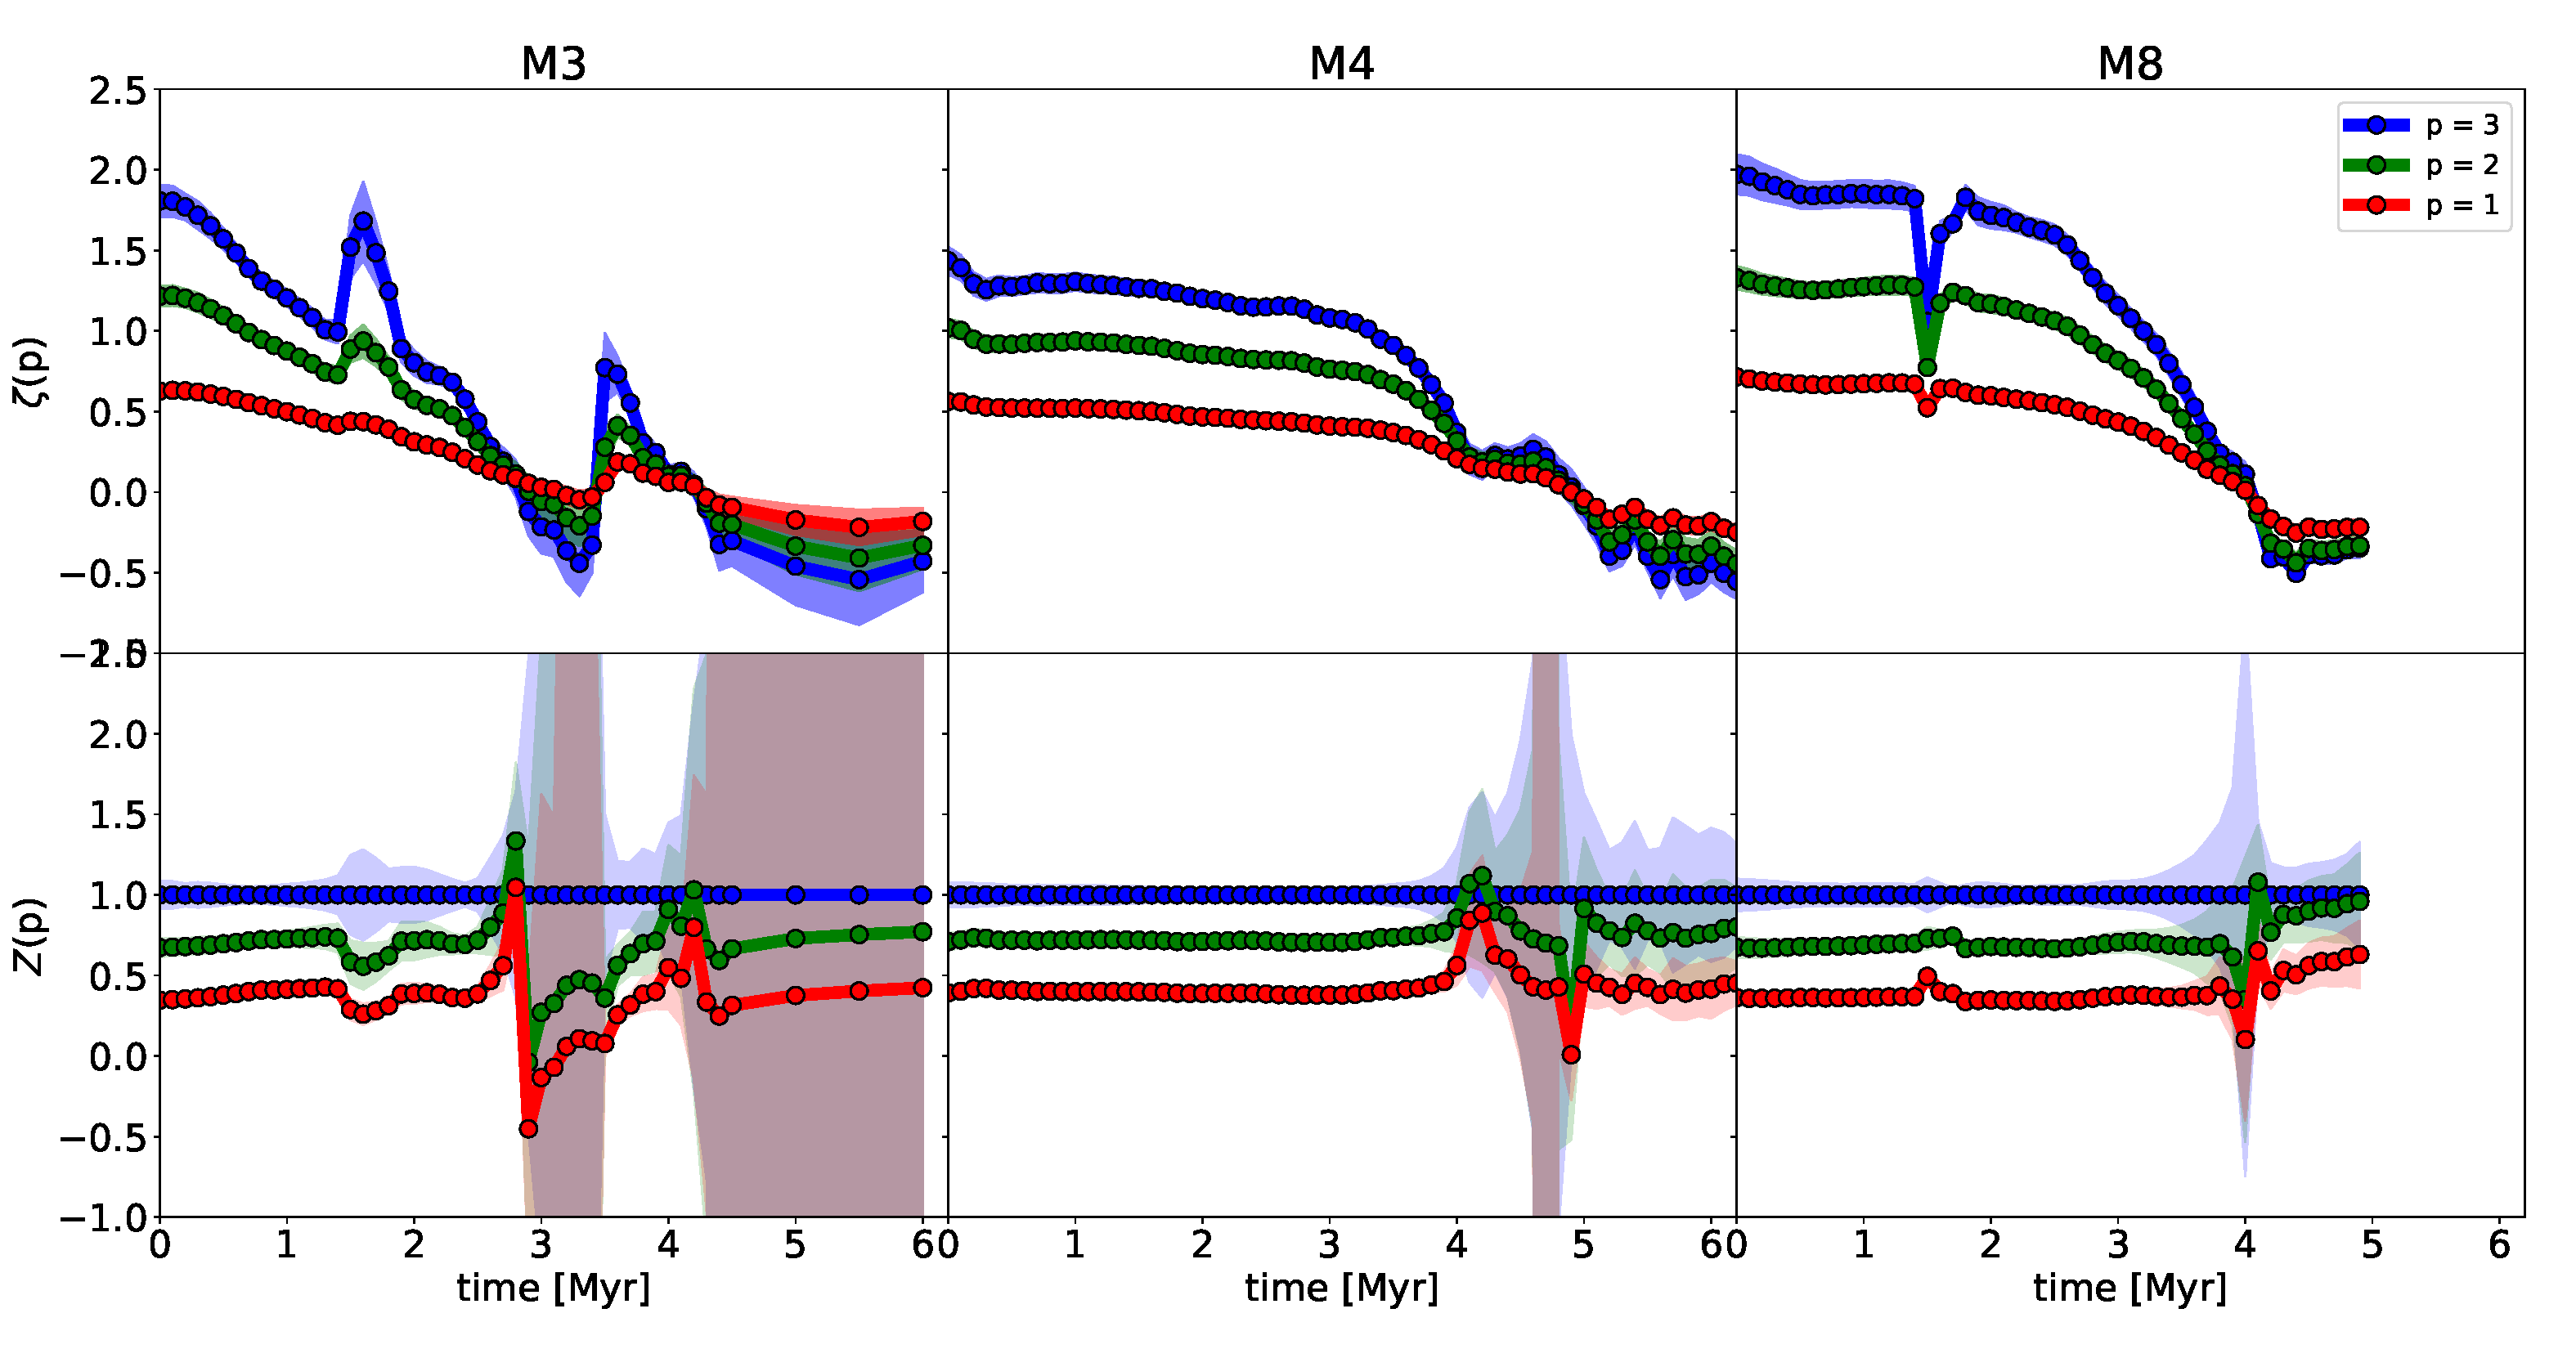
\includegraphics[width=\textwidth]{error_vsf04_zeta_z.pdf}
    \caption{
        Like Fig.~\ref{pic:results:zeta_all}a.
        Additionally, the shaded areas behind the data represent the error ranges of computed $\zeta$ (\textit{top}) and $Z$ (\textit{bottom}), respectively. 
    }
    \label{pic:appFitting:error_vsfhr04_zeta_z}
\end{figure*}






\endinput